\documentclass[a4,12pt]{scrartcl}

%Basic 
\usepackage[utf8]{inputenc}
\usepackage[ngerman]{babel}
\usepackage[T1]{fontenc}
%Schrift 
%\usepackage{fontspec} 
%\setmainfont{Arial} 
%Zeilenabstand
\usepackage{setspace}
\setstretch {1.3}
\usepackage{float}
\usepackage[bottom = 3.50cm]{geometry}

%Titel Seite
\usepackage{titling} %Wird benötigt damit \maketitle die Variabeln title, author und date nicht überschreibt
\title{Domainanalyse}
\subtitle{Projekt: sniffdatel}
\author{David Meister \and Giorgio Vincenti \and Samuel Krieg \and Andreas Stalder}		
 %mit /and können Personen hinzugefügt werden
\date{\today}


%Kopf, Fusszeile
\usepackage{fancyhdr}
\pagestyle{fancy}
\lhead{SW Engineering Projekt FS 2016}
\chead{}
\rhead{sniffdatel}
\lfoot{\thetitle \: v1.0 }
\cfoot{\today }
\rfoot{Seite \thepage}
\renewcommand{\headrulewidth}{0.4pt}

%Bilder
\usepackage{graphicx}

%Zeichnen
\usepackage{tikz}

%Tabellen
\usepackage{booktabs}
\usepackage{longtable}

%Codesnippets
\usepackage{listings}
\lstset{language=java,basicstyle=\footnotesize,frame=single} %backgroundcolor=\color{lightgray}

%Querformat für eine Seite
\usepackage{lscape}
\usepackage{rotating}
\usepackage{pdflscape}

%URL 
\usepackage[colorlinks=true, linkcolor=blue, urlcolor=blue, citecolor=blue]{hyperref}
\urlstyle{same} 


%Loremimpsum
\usepackage{lipsum}



\begin{document}

%\clearpage\maketitle
\begin{titlepage}
	\centering
	\vspace{5cm}
	\begin{center}
	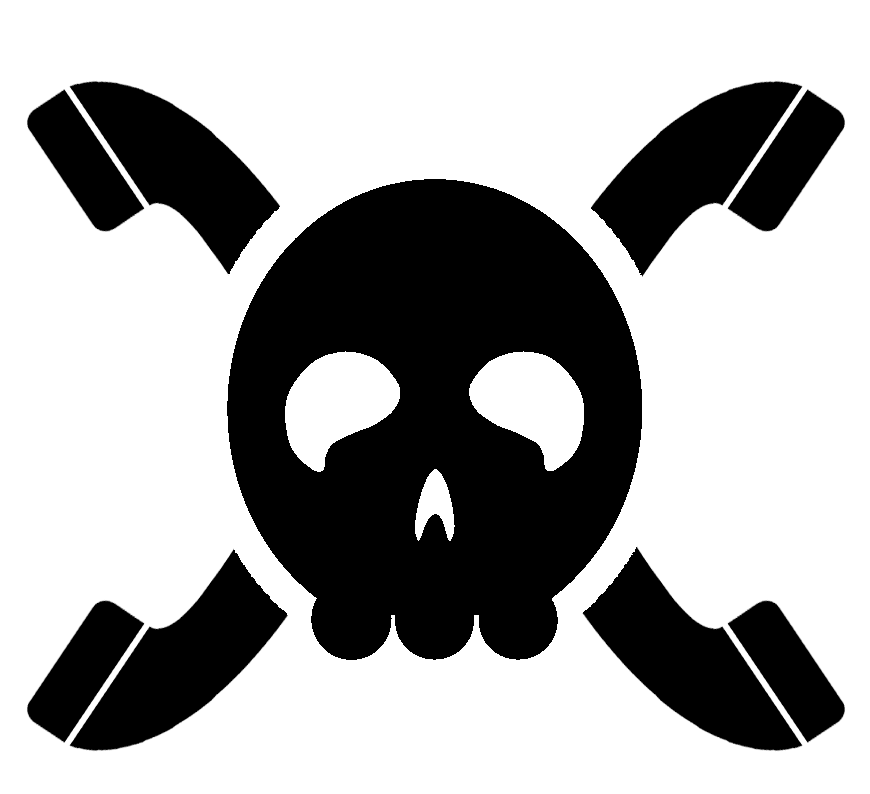
\includegraphics[width=0.50\textwidth]{logo.png}
	\end{center}
	{\huge\bfseries sniffdatel\par}
	\vspace{8cm}
	\raggedright
	{\bfseries SW Engineering Projekt FS 2016\par}
	{\huge\bfseries Domainanalyse\par}
	\vspace{1cm}
	{\theauthor \par}
	{\today\par}

\end{titlepage}

\section{Änderungsgeschichte}

\begin{table}[htb]
\centering
    \begin{tabular}{@{} l l l l@{}}\toprule    
    {Datum} & {Version} & {Änderung} & {Autor}\\ \midrule
    15.03.16 & 1.0 & Erstellung erster Version & Giorgio Vincenti\\ \addlinespace
    16.03.16 & 1.0 & Operation Contracts eingefügt & Giorgio Vincenti\\ \addlinespace
    21.03.16 & 1.0 & Review ready & Alle \\
    %01.03.16 & 1.0 & Vorlage erstellt & Samuel Krieg\\ \addlinespace
    \bottomrule
    \end{tabular}
\caption{\textbf{Änderungsgeschichte}}
\end{table}
\newpage
%\thispagestyle{empty}
\tableofcontents
\newpage


\section{Einführung}
\subsection{Zweck}
Dieses Dokument beschreibt die Problemdomäne mittels eines Domänenmodells, Sequenzdiagrammen und Operation Contracts.
\subsection{Gültigkeitsbereich}
Dieses Dokument ist über die gesamte Projektdauer gültig. Es wird gegebenenfalls in späteren Iterationen angepasst. Somit ist jeweils nur die neuste Version des Dokuments gültigund alte Versionen sind obsolet.
\subsection{Referenzen}
\begin{description}
  Funktionale und Nicht-Funktionale Anforderungen insbesondere Use-Cases. Siehe seperates Dokument.
\end{description}
\newpage


\begin{landscape}
\begin{figure}[htbp]
\section{Domain Modell}
\subsection{Diagramm}
\centering
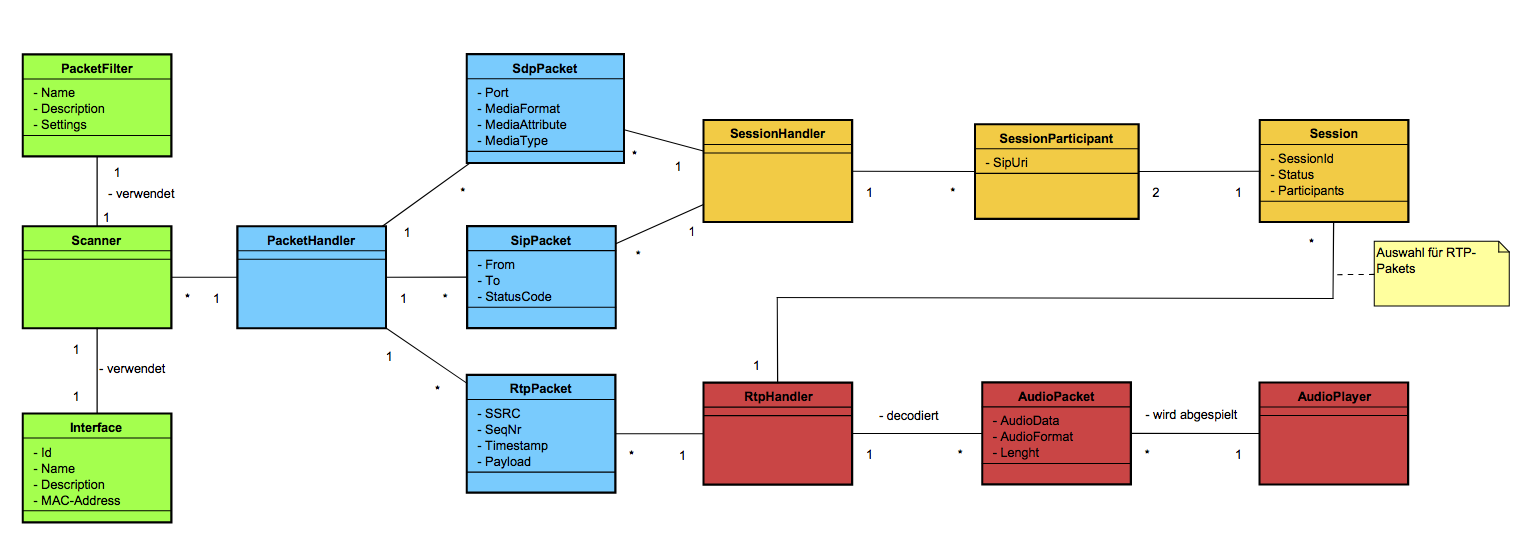
\includegraphics[width=\linewidth, height=\textheight,keepaspectratio]{./figures/DomainModel.png}
\caption{\textbf{Domain Modell}}
\end{figure}
\end{landscape}	
\subsection{Erklärung}
\begin{description}
  \item[PaketFilter] \hfill \\
  Dies ist ein selbst programmiertes Filterobjekt, welches dem Scanner übergeben werden kann. 
  \item[Scanner] \hfill \\
  Zeichnet Pakete auf Interface auf und leitet diese an den PaketHandler weiter.
  \item[Device] \hfill \\
  Objekt, welches physikalisches Netzwerkinterface abbildet.
  \item[PaketHandler] \hfill \\
  Wandelt Raw Pakets in formatierte Paketobjekte um.
  \item[SdpPaket] \hfill \\
  Paketobjekt für SDP Pakete
  \item[SipPaket] \hfill \\
  Paketobjekt für SIP Pakete
  \item[RtpPaket] \hfill \\
  Paketobjekt für RTP Pakete
  \item[SessionFinder] \hfill \\
  Erzeugt aus erhaltenen SIP und SDP Paketen Sessions
  \item[Session] \hfill \\
  Sessionobjekt, beinhaltet die Session ID, Sessionstatus und die Teilnehmer
  \item[PaketDecoder] \hfill \\
  Decodiert RTP Pakete für ausgewählte Sessions
  \item[AudioPaket] \hfill \\
  Abspielbares Audioobjekt
  \item[AudioPlayer] \hfill \\
  Spielt erhaltene Audiopakete ab.
\end{description}

\section{Systemsequenzdiagramme}
\subsection{Use Case 1: Select Interface}
\begin{figure} [H]
	\begin{center}
	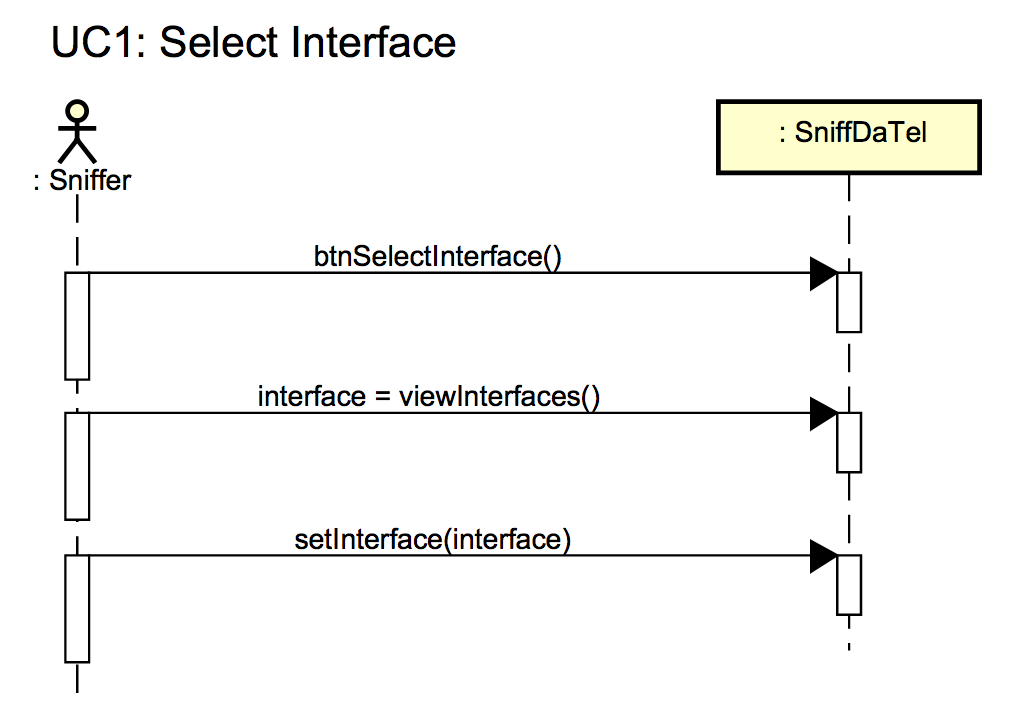
\includegraphics[width=0.60\textwidth]{./figures/UC1.png}
	\caption{\textbf{SSD Select Interface}}
	\label{Bild Referenz}
	\end{center}
\end{figure}

\subsection{Use Case 2: Collecting Sessions}
\begin{figure} [H]
	\begin{center}
	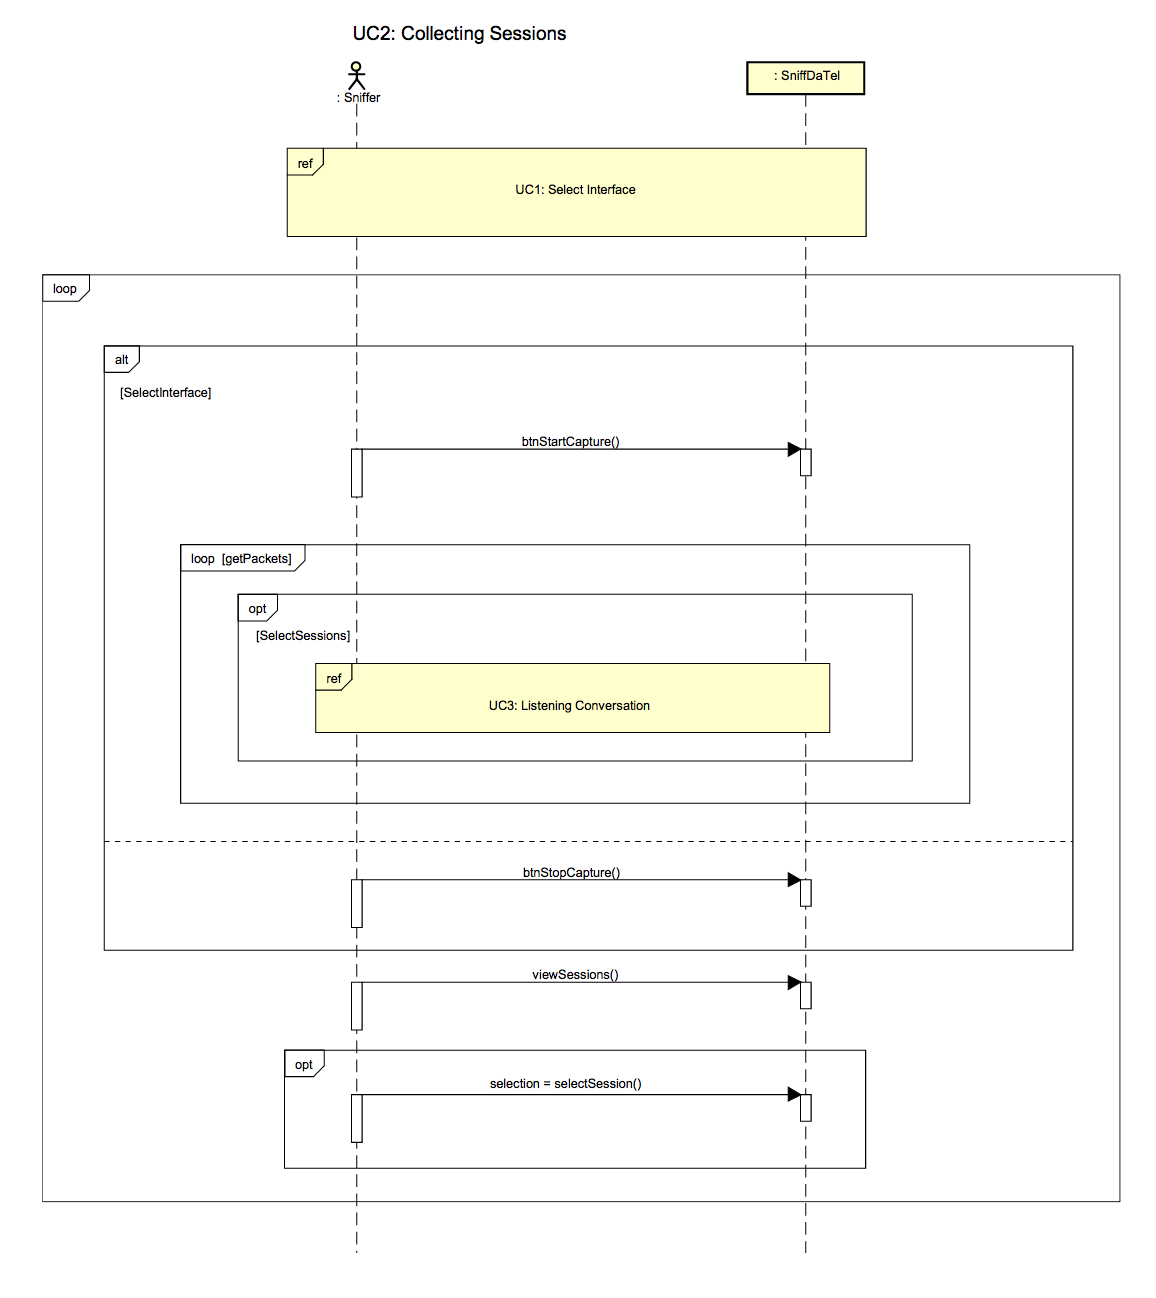
\includegraphics[width=\textwidth]{./figures/UC2.png}
	\caption{\textbf{SSD Collecting Sessions}}
	\label{Bild Referenz}
	\end{center}
\end{figure}

\subsection{Use Case 3: Listening Conversation}
\begin{figure} [H]
	\begin{center}
	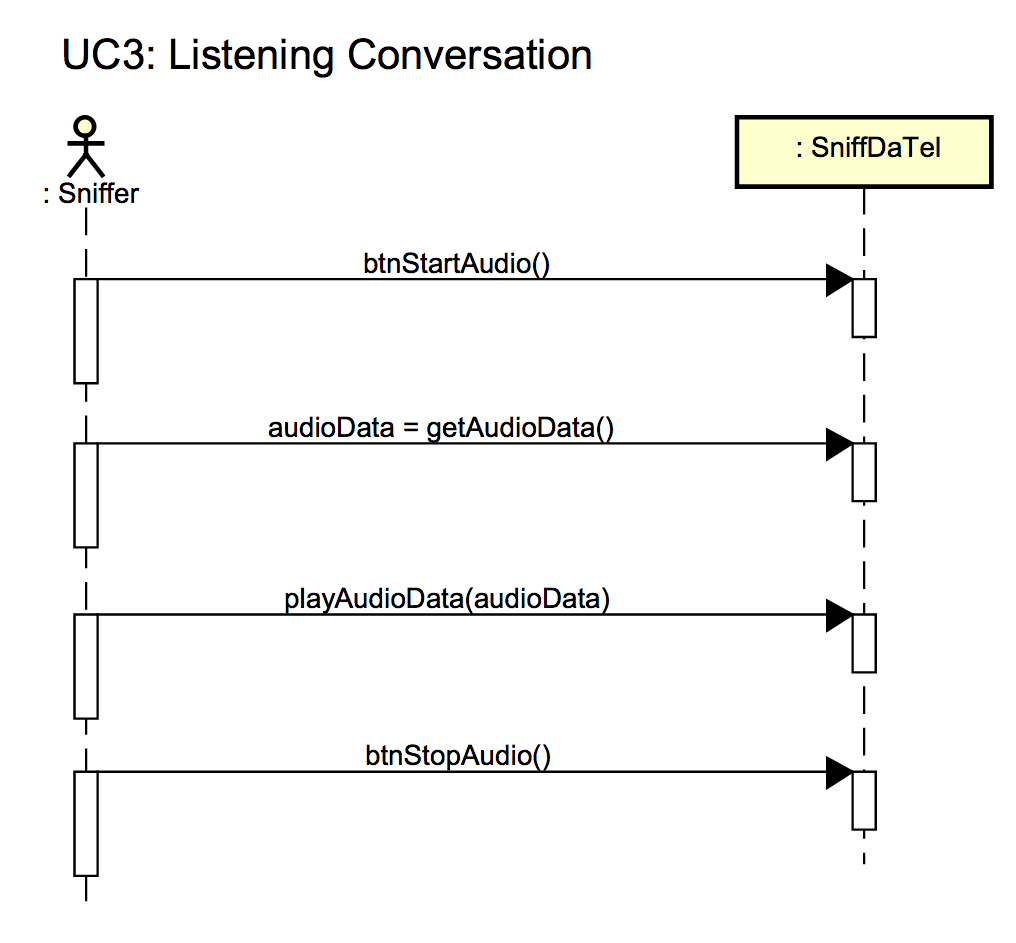
\includegraphics[width=0.60\textwidth]{./figures/UC3.png}
	\caption{\textbf{SSD Listening Conversation}}
	\label{Bild Referenz}
	\end{center}
\end{figure}

\section{Systemoperationen}
\subsection{Vertrag Systemoperation1: viewInterfaces()}
\begin{table}[H]
\centering
    \begin{tabular}{@{} l l@{}}    
    {Position} & {Description}\\ \midrule
   	Systemoperation & viewInterfaces()\\ \addlinespace
   	Beschreibung & Liefert alle Netzwerk Interfaces\\ \addlinespace
   	Precondition & Eine Instanz availableInterfaces von Interface existiert\\ \addlinespace
	Postcondition & Interface Liste in availableInterfaces gespeichert\\ \addlinespace
	& availableInterfaces angezeigt\\ \bottomrule
    \end{tabular}
\caption{\textbf{Systemoperation1}}
\end{table}
\subsection{Vertrag Systemoperation2: setInterfaces(interface)}
\begin{table}[H]
\centering
    \begin{tabular}{@{} l l@{}}    
    {Position} & {Description}\\ \midrule
   	Systemoperation & setInterfaces(interface)\\ \addlinespace
   	Beschreibung & Sniffer wählt gewünschtes Interface aus Liste\\ \addlinespace
   	Precondition & Eine Instanz currentInterface von Interface existiert\\ \addlinespace
	Postcondition & Instanzvariablen von currentInterface wurden gesetzt\\
	\addlinespace
	& currentInterface verknüpft mit Scannerinstanz\\ \bottomrule
    \end{tabular}
\caption{\textbf{Systemoperation2}}
\end{table}

\subsection{Vertrag Systemoperation3: btnSelectInterface()}
\begin{table}[H]
\centering
    \begin{tabular}{@{} l l@{}}    
    {Position} & {Description}\\ \midrule
   	Systemoperation & btnSelectInterface() \\ \addlinespace
   	Referenz & Use Case (UC1) select interface\\ \addlinespace
   	Beschreibung & Sniffer drückt auf Button "capture interfaces". \\ \addlinespace
   	Precondition & Main GUI Instanz ist erstellt\\ \addlinespace
	Postcondition & Caputure Interfaces GUI Instanz wurde erstellt.\\ \bottomrule
    \end{tabular}
\caption{\textbf{Systemoperation3}}
\end{table}

\subsection{Vertrag Systemoperation4: btnStartCapture()}
\begin{table}[H]
\centering
    \begin{tabular}{@{} l l@{}}    
    {Position} & {Description}\\ \midrule
   	Systemoperation & btnStartCapture()\\ \addlinespace
   	Beschreibung & Sniffer drückt auf Button start capture.\\ \addlinespace
   	Precondition & Interface Instanz currentInterface muss vorhanden sein. \\ \addlinespace
   	& Filter Instanz filter muss vorhanden sein. \\ \addlinespace
   	& PaketHandler Instanz paketHandler muss vorhanden sein. \\ \addlinespace
	Postcondition & scanner übergibt Pakete an paketHandler\\ \bottomrule
    \end{tabular}
\caption{\textbf{Systemoperation4}}
\end{table}
\subsection{Vertrag Systemoperation5: btnStopCapture()}
\begin{table}[H]
\centering
    \begin{tabular}{@{} l l@{}}    
    {Position} & {Description}\\ \midrule
   	Systemoperation & btnStopCapture()\\ \addlinespace
   	Beschreibung & Sniffer drückt auf Button "stop capture".\\ \addlinespace
   	Precondition & Interface Instanz currentInterface muss vorhanden sein. \\ \addlinespace
   	& Filter Instanz filter muss vorhanden sein. \\ \addlinespace
   	& PaketHandler Instanz paketHandler muss vorhanden sein. \\ \addlinespace
	Postcondition & Scanner gestopt \\ \bottomrule
    \end{tabular}
\caption{\textbf{Systemoperation5}}
\end{table}
\subsection{Vertrag Systemoperation6: viewSessions()}
\begin{table}[H]
\centering
    \begin{tabular}{@{} l l@{}}    
    {Position} & {Description}\\ \midrule
   	Systemoperation & view Sessions()\\ \addlinespace
   	Beschreibung & Sniffdatel zeigt dem Sniffer die gefundenen VoIP Sessions an. \\ \addlinespace
   	Precondition & SessionHandler sessionHandler muss instanziert sein.\\ \addlinespace
	Postcondition & Session Instanz session wurde instanziert. \\ \addlinespace
	& Instanzvariablen von session wurden gesetzt
	\\ \bottomrule
    \end{tabular}
\caption{\textbf{Systemoperation6}}
\end{table}
\subsection{Vertrag Systemoperation7: selectSession()}
\begin{table}[H]
\centering
    \begin{tabular}{@{} l l@{}}    
    {Position} & {Description}\\ \midrule
   	Systemoperation & selectSessions()\\ \addlinespace
   	Beschreibung & Sniffer wählt eine gefundene Session aus.\\ \addlinespace
   	Precondition & Session Instanz session wurde instanziert. \\ \addlinespace
	Postcondition & Ausgewählte Session wurde in currentSession gespeichert\\ \bottomrule
    \end{tabular}
\caption{\textbf{Systemoperation7}}
\end{table}
\subsection{Vertrag Systemoperation8: btnStartAudio()}
\begin{table}[H]
\centering
    \begin{tabular}{@{} l l@{}}    
    {Position} & {Description}\\ \midrule
   	Systemoperation & btnStartAudio()\\ \addlinespace
   	Referenz & Use Case (UC3) listening conversation\\ \addlinespace
   	Beschreibung & Sniffer drückt auf Button "start audio"\\ \addlinespace
   	Precondition & Instanz audioPlayer existiert. \\ \addlinespace
   	& Instanz audioPaket existiert\\ \addlinespace 
	Postcondition & audioPaket wurde an audioPlayer übergeben\\ 
	\bottomrule
    \end{tabular}
\caption{\textbf{Systemoperation8}}
\end{table}
\subsection{Vertrag Systemoperation9: btnStopAudio()}
\begin{table}[H]
\centering
    \begin{tabular}{@{} l l@{}}    
    {Position} & {Description}\\ \midrule
   	Systemoperation &  btnStopAudio()\\ \addlinespace
   	Beschreibung & Sniffer drückt auf Button "stop audio".\\ \addlinespace
   	Precondition & Instanz audioPlayer existiert\\ \addlinespace
	Postcondition & audioPlayer.stop() ausgeführt\\ \bottomrule
    \end{tabular}
\caption{\textbf{Systemoperation9}}
\end{table}
\subsection{Vertrag Systemoperation10: getAudioData()}
\begin{table}[H] 
\centering
    \begin{tabular}{@{} l l@{}}    
    {Position} & {Description}\\ \midrule
   	Systemoperation & getAudioData()\\ \addlinespace
   	Beschreibung & Pakete mit VoIP Inhalte werden in die Variable audioData gespeichert.\\ \addlinespace
   	Precondition & rtpHandler Instanz existiert\\ \addlinespace
	Postcondition & rtpHandler speichert RTP Payload in ein AudioPaket\\ \bottomrule
    \end{tabular}
\caption{\textbf{Systemoperation11}}
\end{table}
\subsection{Vertrag Systemoperation11: playAudio(audioData)}
\begin{table}[H]
\centering
    \begin{tabular}{@{} l l@{}}    
    {Position} & {Description}\\ \midrule
   	Systemoperation & playAudio(audioData)\\ \addlinespace
   	Beschreibung & Wiedergabe der Inhalte der Variable audioData. \\ \addlinespace
   	Precondition & Audio Paket Instanz audioPaket muss existieren.\\ \addlinespace
	Postcondition & audioPaket wurde an audioPlayer übergeben\\ \bottomrule
    \end{tabular}
\caption{\textbf{Systemoperation12}}
\end{table} 
\subsection{Vertrag Systemoperation12: stopAudio()}
\begin{table}[H]
\centering
    \begin{tabular}{@{} l l@{}}    
    {Position} & {Description}\\ \midrule
   	Systemoperation & stopAudio()\\ \addlinespace
   	& Use Case (UC2) collecting sessions \\ \addlinespace
   	Beschreibung & Sniffer drückt auf Button "stop audio".\\ \addlinespace
   	Precondition & audioPlayer instanz existiert\\ \addlinespace
	Postcondition & audioPlayer.stop() ausgeführt\\ \bottomrule
    \end{tabular}
\caption{\textbf{Systemoperation13}}
\end{table}

\begin{landscape}
\begin{figure}[htbp]
\section{Zustandsdiagramm}
\centering
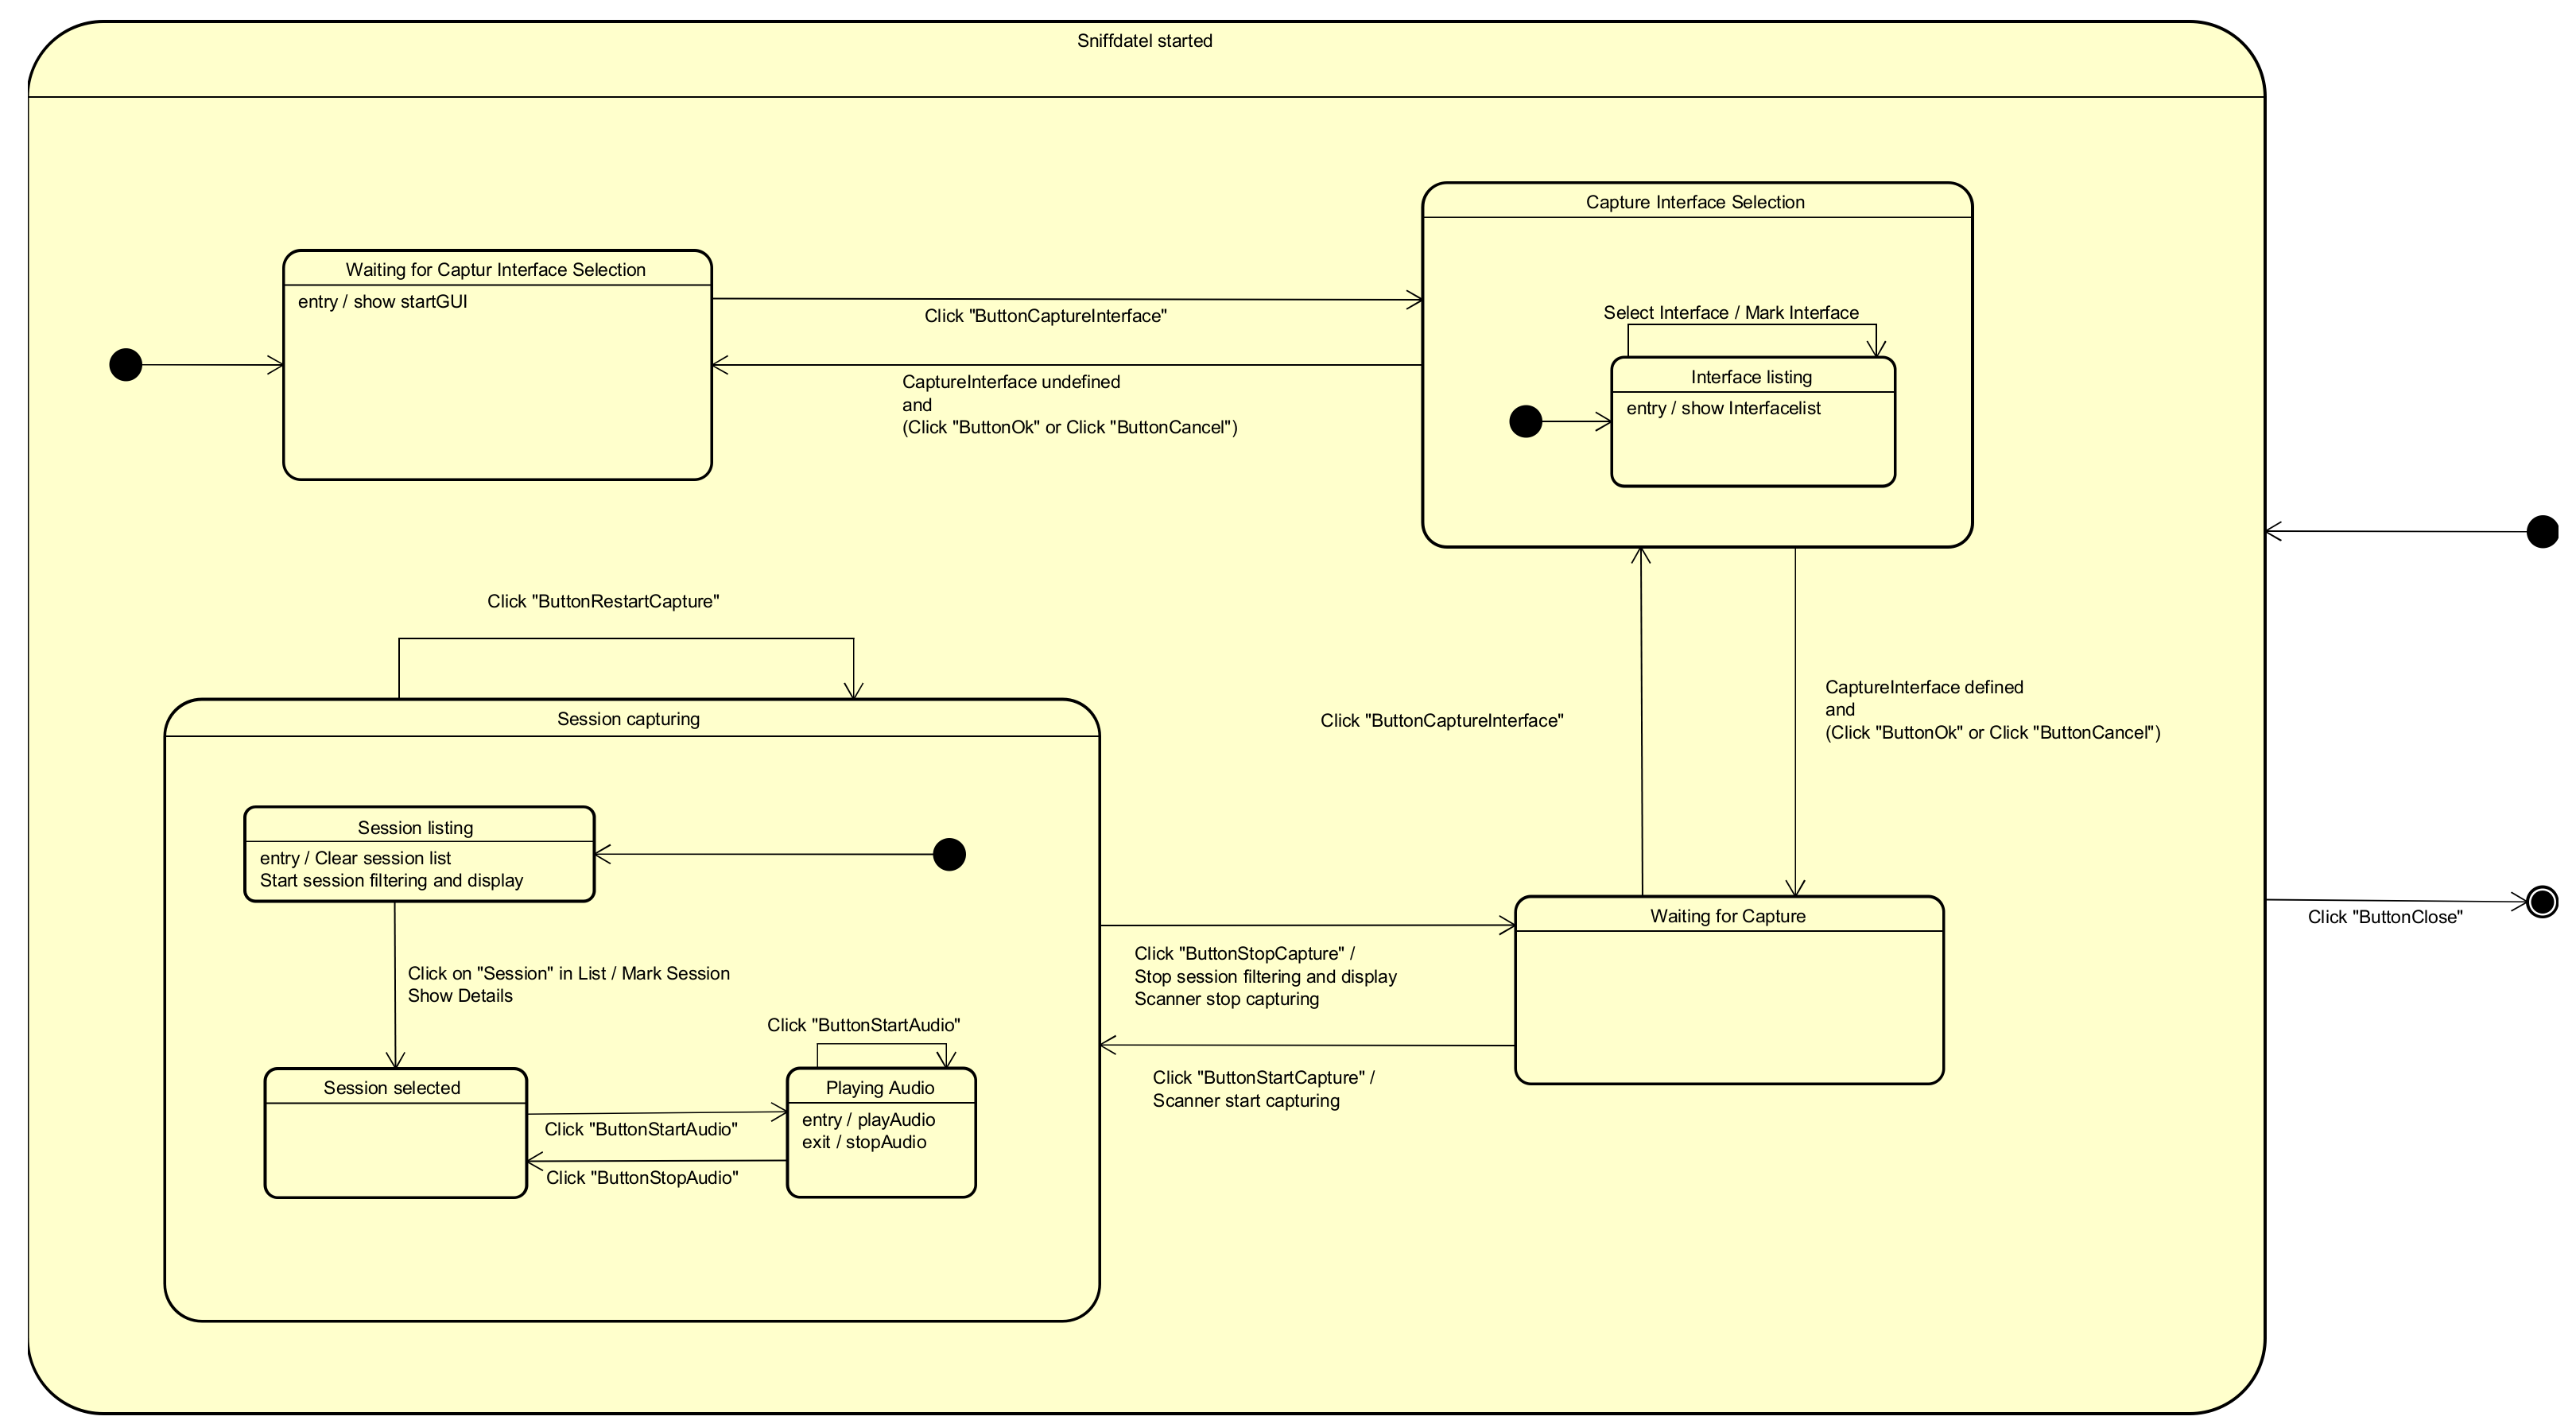
\includegraphics[width=\linewidth, height=\textheight,keepaspectratio]{./figures/Statemachine.png}
\caption{\textbf{Zustandsdiagramm}}
\end{figure}
\end{landscape}	

\section{Activity Diagramm}
\begin{figure} [H]
	\begin{center}
	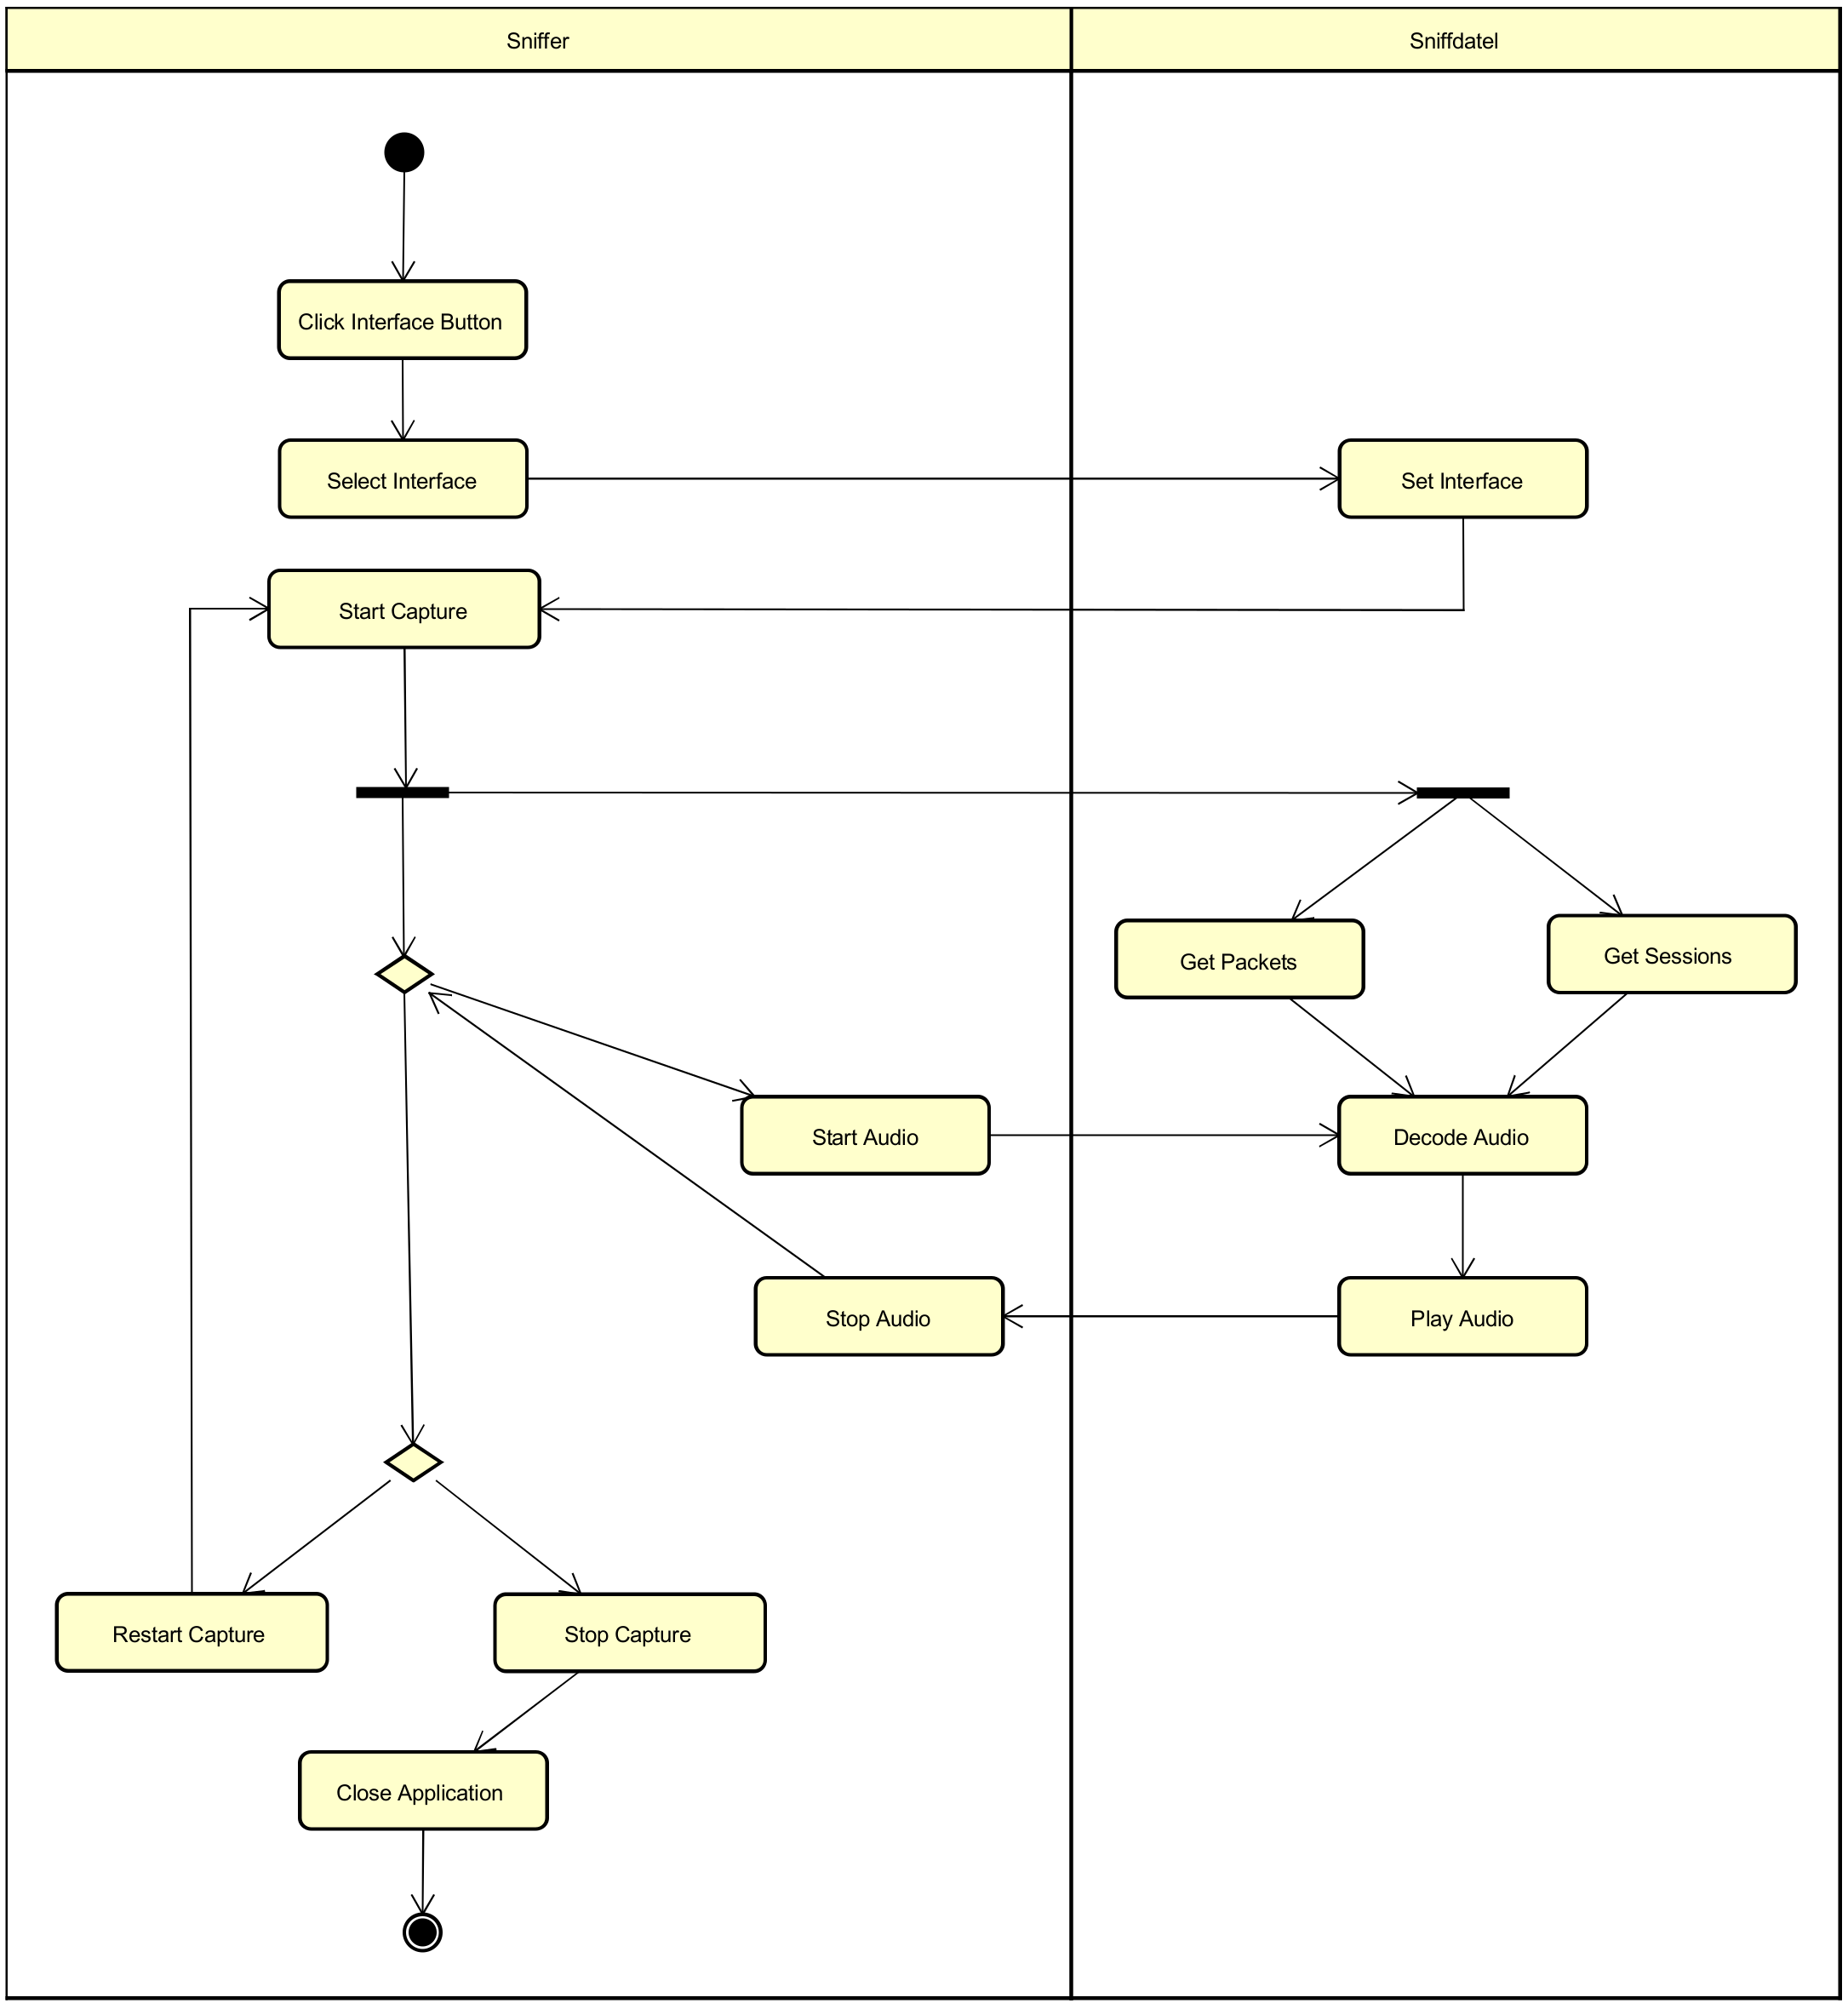
\includegraphics[width=\textwidth]{./figures/ActivityDiagram.png}
	\caption{\textbf{Activity Diagramm}}
	\label{Bild Referenz}
	\end{center}
\end{figure}

\end{document}

